\section{Aplicare pe setul de date}

\subsection{Problema pe care o rezolvăm}
Așa cum am precizat și în primul capitol, problema pe care o abordez este una de învățare multi-instanță și învâțare multi-etichetă. \\

O instanță este o fotografie dintr-un restaurant, însă noi vom clasifica un întreg restaurant folosindu-ne de pozele făcute în acesta. De aici vine caracterul multi-instanță a problemei, iar cel multi-etichetă este dat de faptul că, pentru un restaurant, va trebui să răspundem cu adevărat/fals la 9 întrebări, oferindu-i etichetele aferente:

\begin{enumerate}
\item bun pentru prânz (good for lunch)
\item bun pentru cină (good for dinner)
\item acceptă rezervări (takes reservations)
\item are sejur în aer liber (outdoor seating)
\item este scump (restaurant is expensive)
\item oferă alcool (has alcohol)
\item are serviciu de masă (has table service)
\item atmosfera este rustică (ambience is classy)
\item bun pentru copii (good for kids)
\end{enumerate}

\subsection{Abordare}
Vom reaminti structura setului de date pus la dispoziție.

\begin{itemize}
\item 234842 de imagini de antrenament în format .jpg și .png.
\item 237152 de imagini de test.
\item \textit{\textbf{train\_photo\_to\_biz\_ids.csv}}: tabel ce asociază fiecare fotografie de antrenament la restaurantul din care provine folosind id-uri.
\item \textit{\textbf{train.csv}}: tabel ce conține 2 coloane $\{business\_id, labels\}$ semnificând etichetarea unui restaurant (prin id-ul său) cu o submulțime din $\{1,2,...,9\}$ ce reprezintă cele 9 clase ilustrate mai sus.
\item \textit{\textbf{test\_photo\_to\_biz\_ids.csv}}: tabel ce asociază fiecare fotografie de test la restaurantul din care provine folosind id-uri.
\end{itemize}

În total sunt 1996 de restaurante în setul de antrenament și 10000, ce trebuie clasificate, în setul de testare.

În abordarea mea, am adoptat un pipeline simplu, format din 4 pași secvențiali:

\begin{itemize}
\item Preprocesare date.
\item Extragerea de caracteristici și construirea unui vector caracteristic pentru fiecare restaurant.
\item Antrenarea unui model pentru a clasifica restaurantele.
\item Evaluarea rezultatelor.
\end{itemize}

\begin{center}
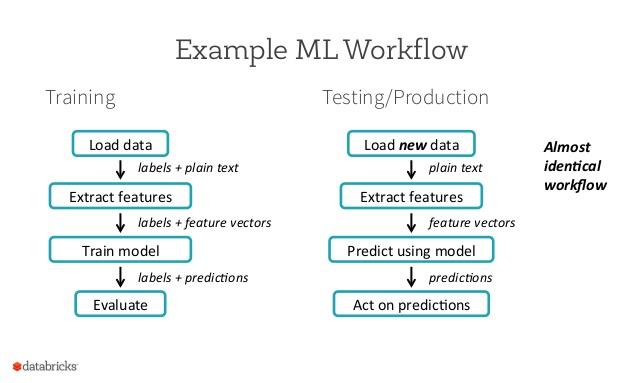
\includegraphics[scale=0.6]{pipeline} \\
Figura 31: Workflow pentru antrenare și testare
\end{center}

\subsubsection{Prelucrare date}
În această etapă am eliminat inconsistențele din date (fotografii ce nu aveau niciun restaurant asociat sau restaurante ce nu aveau fotografii) și am adus toate imaginile la rezoluția 299x299 ce corespunde marimii input-ului pentru modelul Xception pe care l-am folosit pentru extragerea de caracteristici.

\subsubsection{Extragerea de caracteristici}
Pentru fiecare imagine de mărime 299x299 introdusă în modelul Xception, obținem un vector caracteristic cu 2048 de componente dacă extragem datele prelucrate de model la penultimul layer, înaintea celui de clasificare. Astfel, fiecare imagine din setul de antrenament va fi reprezentată de către un vector din $\mathbb{R}^{2048}$. Scopul nostru însă, este să clasificăm restaurantele, nu fiecare poză în parte, așa că, pentru fiecare restaurant, vom combina vectorii caracteristici a fiecărei fotografii din acesta, recurgând la calcularea medii aritmetice pentru acești vectori. După executarea acestui pas, setul nostru de date va avea forma $(1996,2048)$, având pentru fiecare restaurant câte un vector de 2048 de componente și folosind PCA (Principal Component Analysis) putem vizualiza acești vectori (\textcolor{yellow}{GALBEN} - clasa este prezentă, \textcolor{purple}{MOV} - clasa este absentă).

\begin{center}
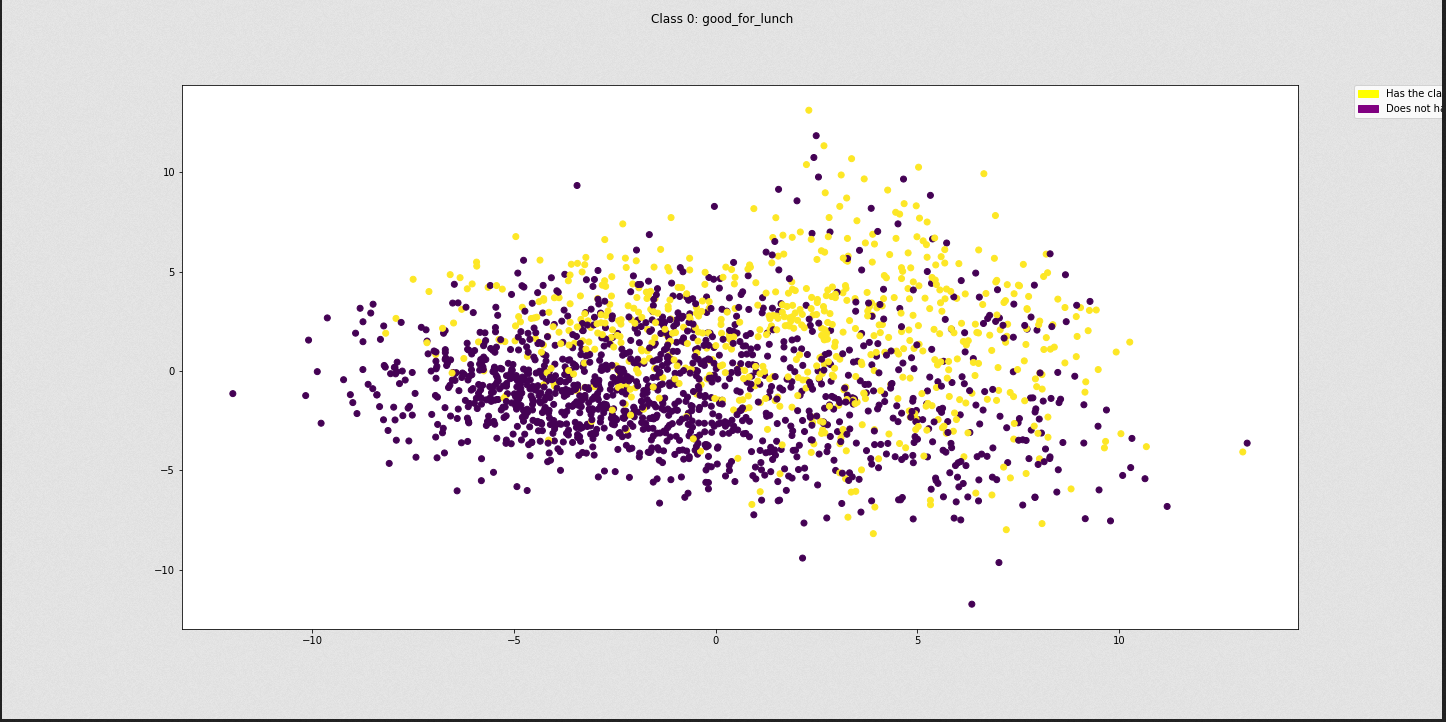
\includegraphics[scale=0.4]{class0} \\
Figura 32: Grafic pentru prima clasă: bun pentru prânz \\
\hfill \break

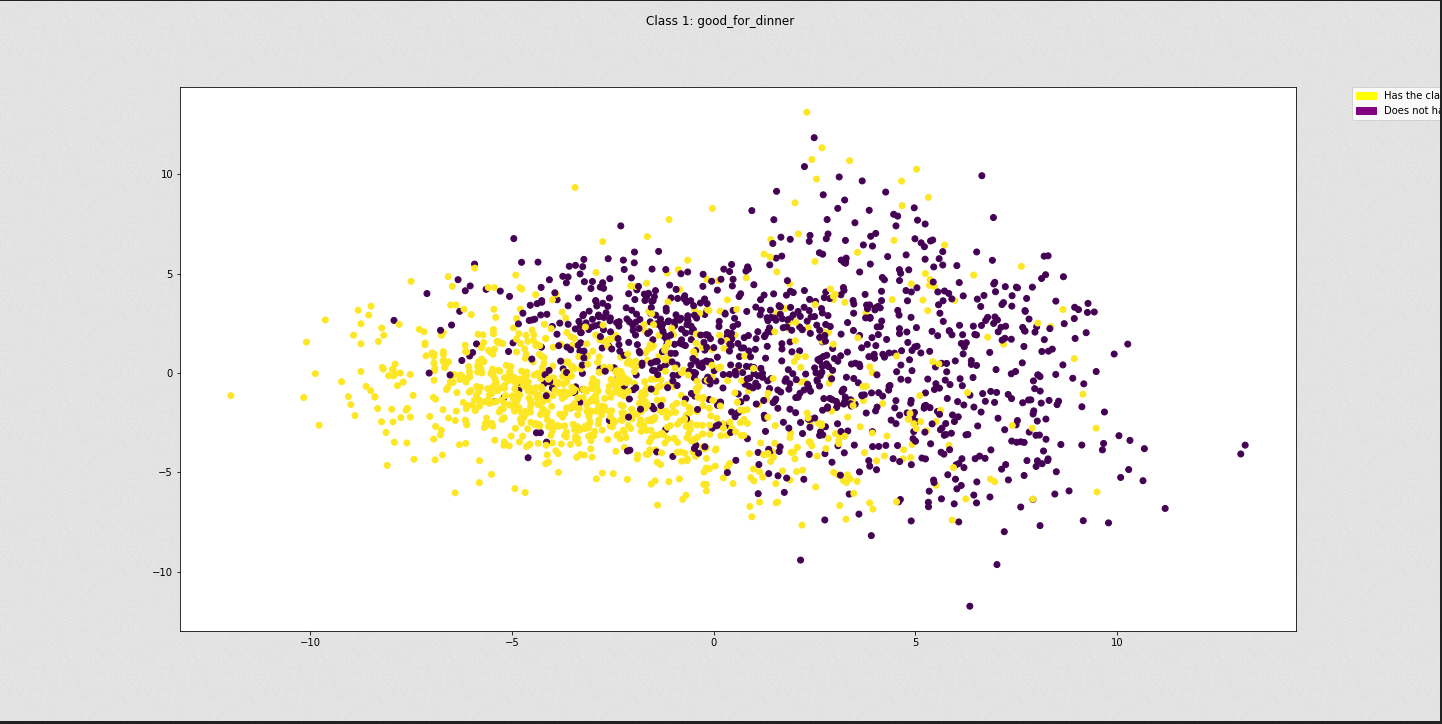
\includegraphics[scale=0.4]{class1} \\
Figura 33: A doua clasă: bun pentru cină \\
\hfill \break

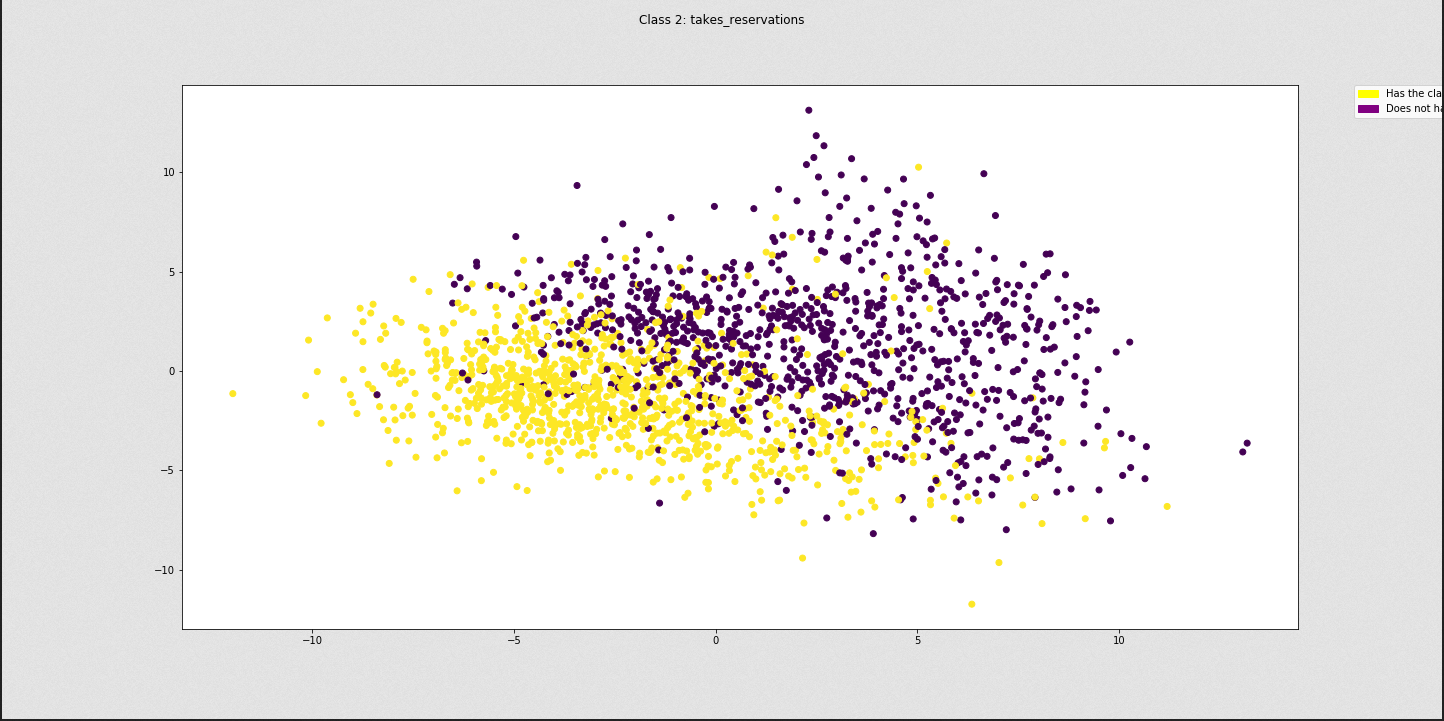
\includegraphics[scale=0.4]{class2} \\ 
Figura 34: A treia clasă: acceptă rezervări \\ 
\hfill \break

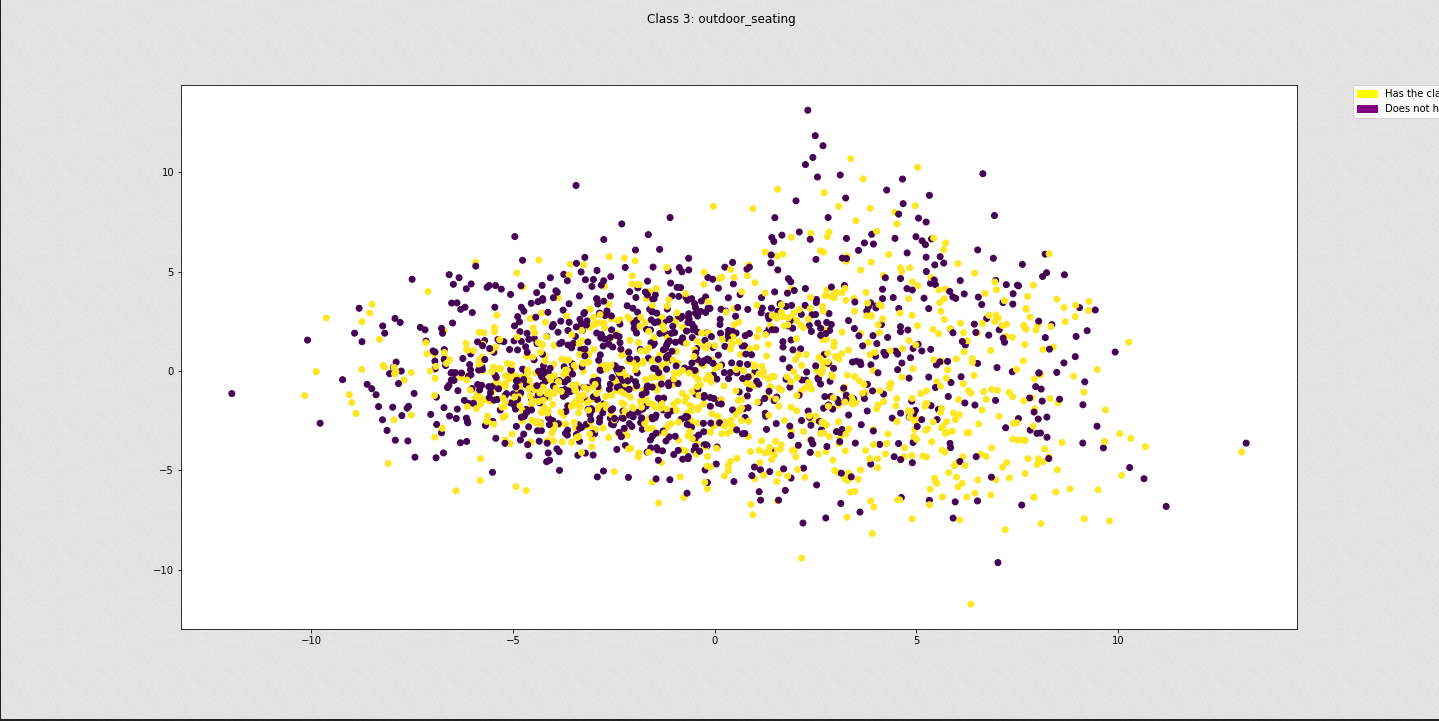
\includegraphics[scale=0.4]{class3} \\
Figura 35: A patra clasă: are sejur în aer liber \\
\hfill \break

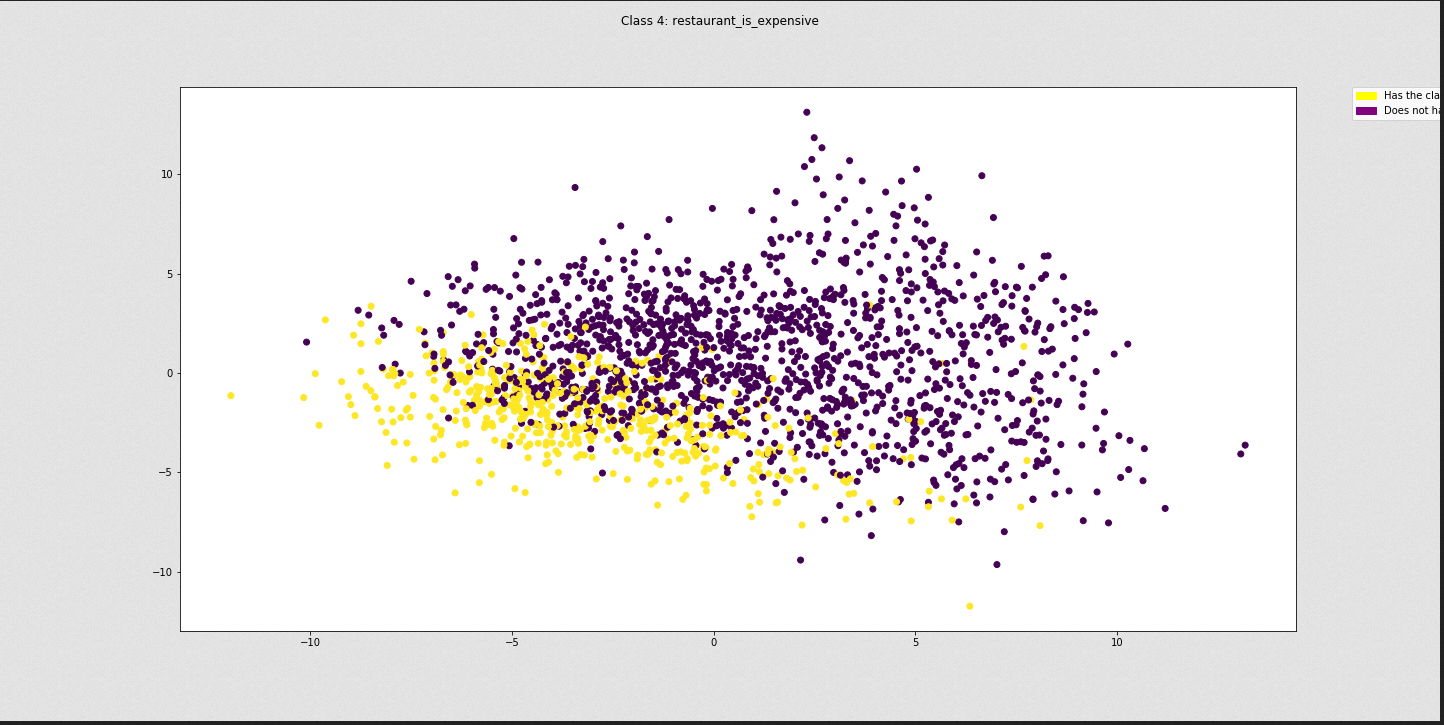
\includegraphics[scale=0.4]{class4} \\
Figura 36: A cincea clasă: este scump \\
\hfill \break

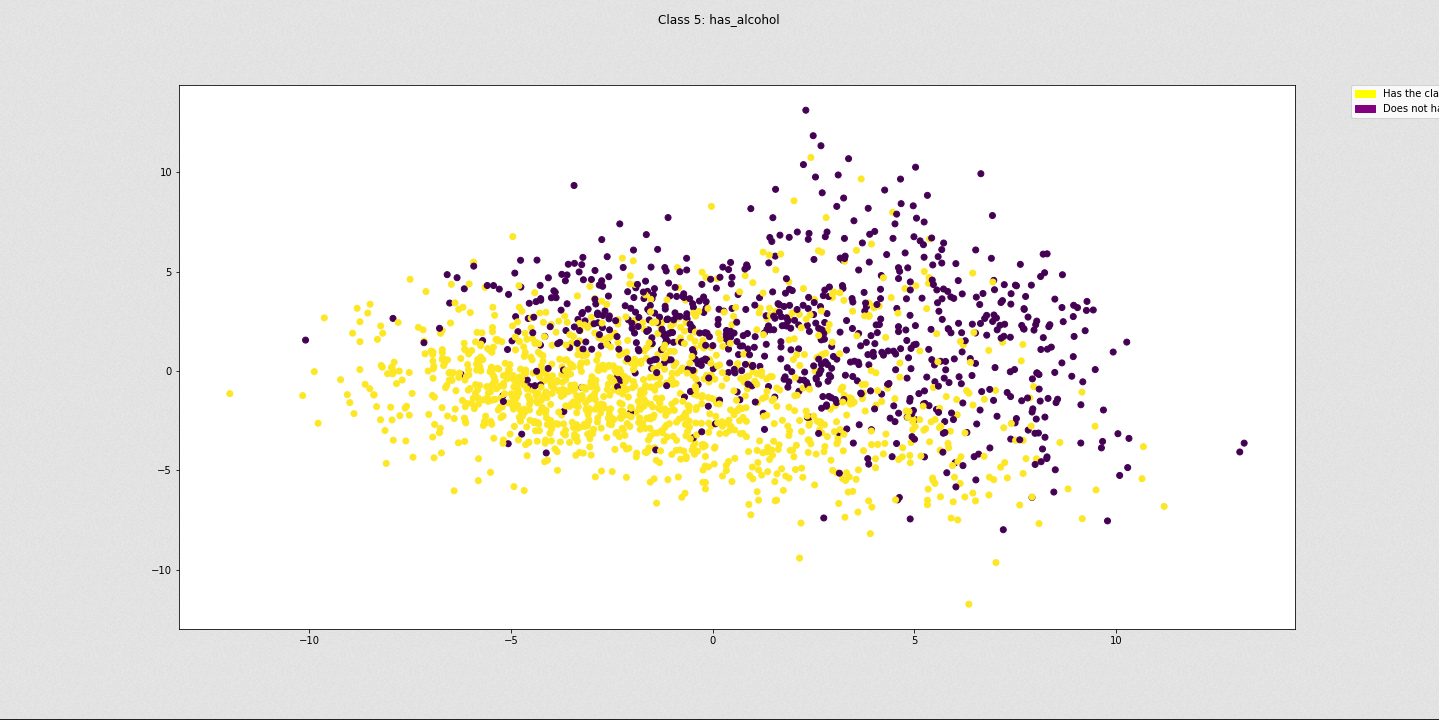
\includegraphics[scale=0.4]{class5} \\
Figura 37: A șasea clasă: oferă alcool \\
\hfill \break

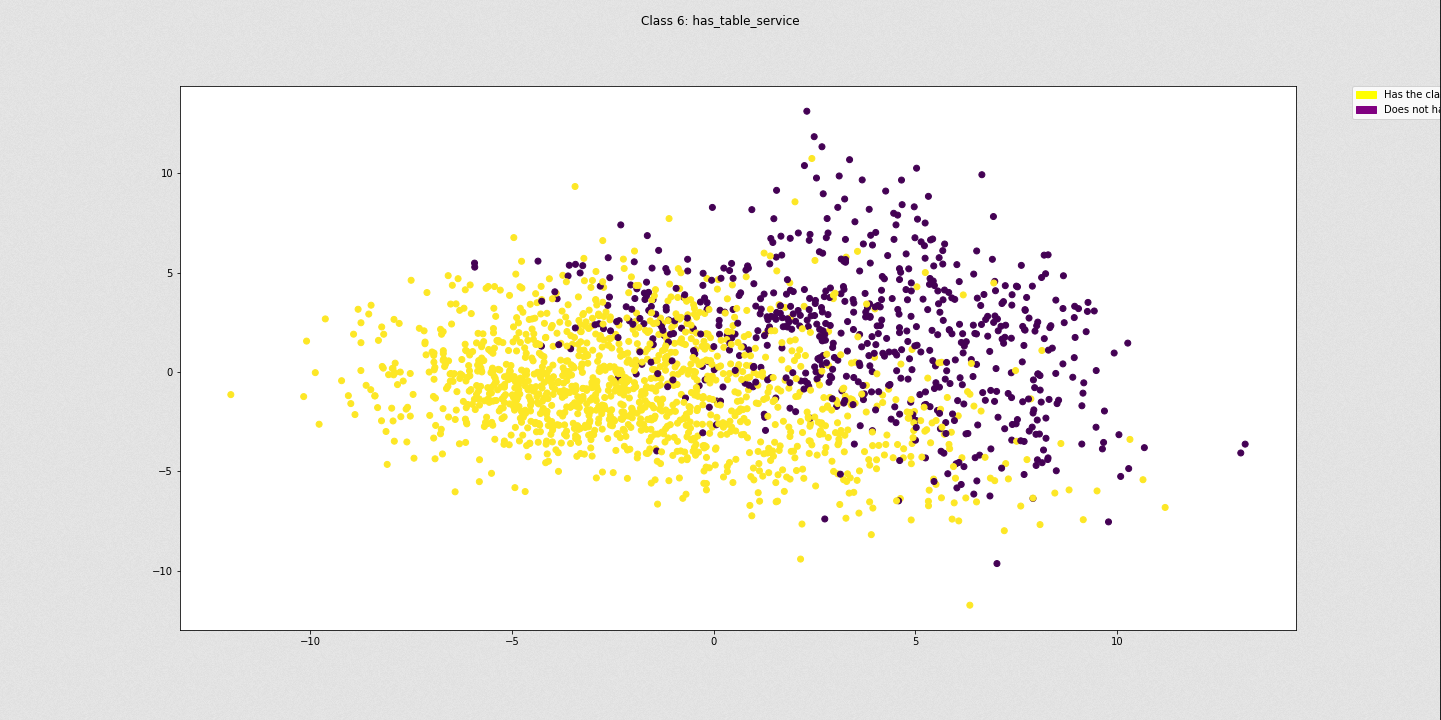
\includegraphics[scale=0.4]{class6} \\
Figura 38: A șaptea clasă: are serviciu de masă \\
\hfill \break

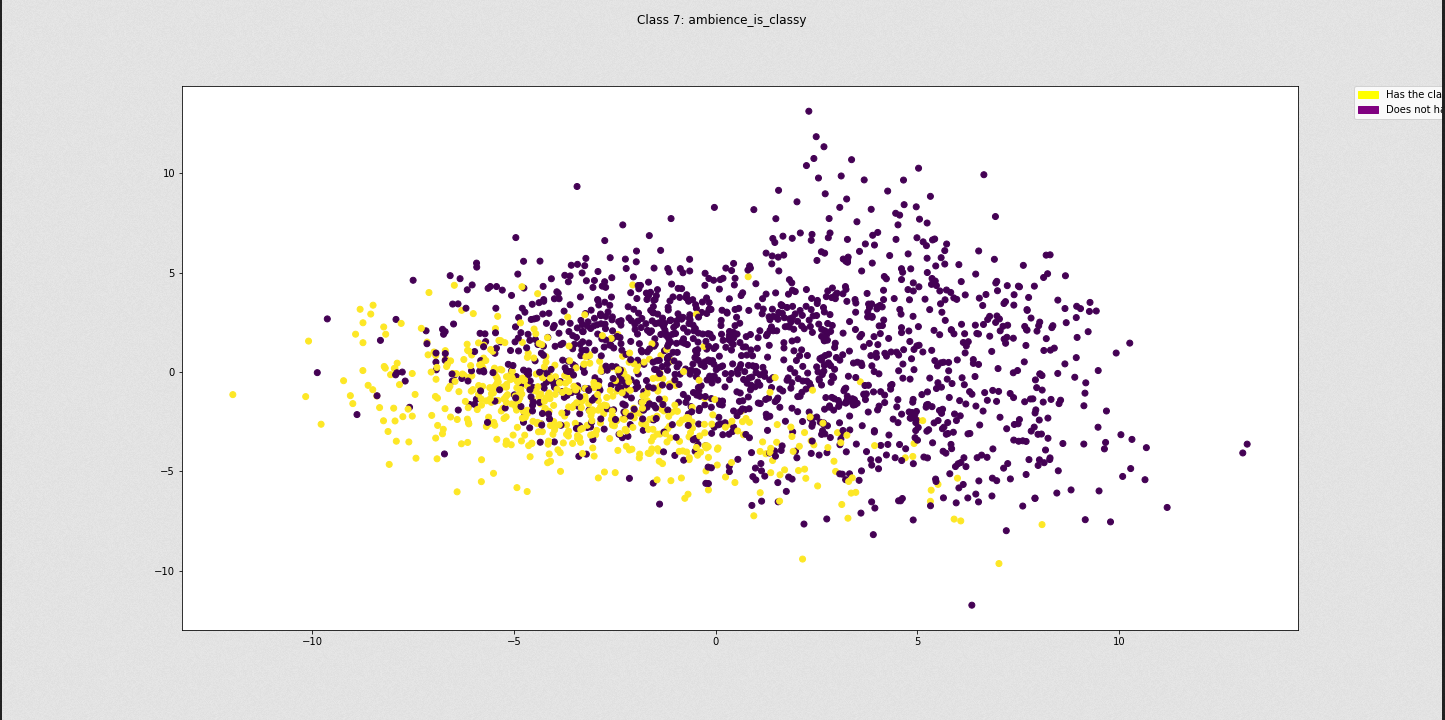
\includegraphics[scale=0.4]{class7} \\
Figura 39: A opta clasă: atmosfera este rustică \\
\hfill \break

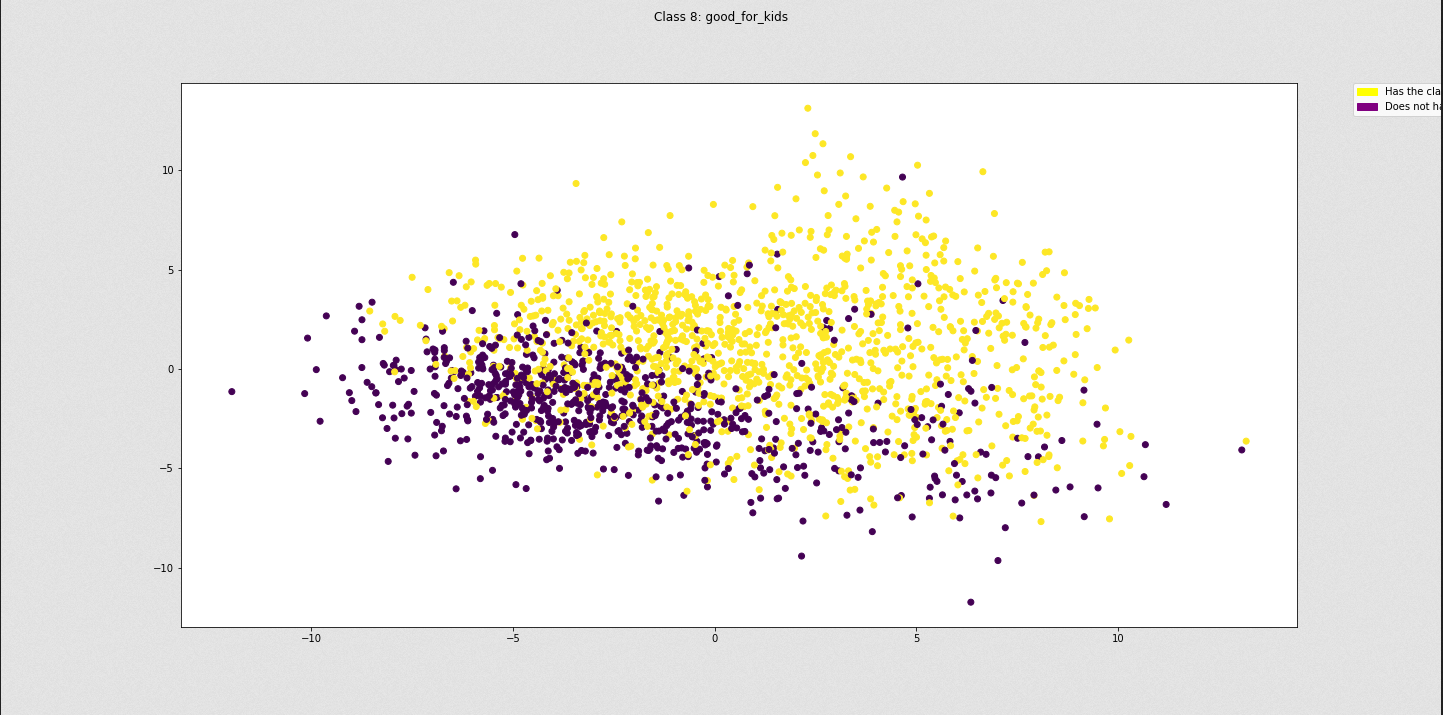
\includegraphics[scale=0.4]{class8} \\
Figura 40: A noua clasă: bun pentru copii \\
\end{center}

\pagebreak

Pentru setul de date de forma $(1996,2048)$ am adoptat o rețea neuronală clasică cu 3 hidden layers de marimi $\{2500,1024,365\}$, activări $ReLU/LeakyReLU$ și cu o valoare pentru Dropout de $0.5$.

\begin{center}
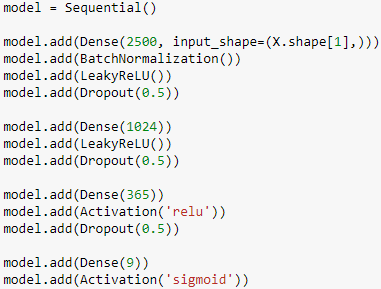
\includegraphics[scale=1]{networkArhitecture} \\
Figura 41: Cod Python ce instanțiază modelul
\end{center}

\subsection{Detalii de implementare}
Pentru implementarea întregului pipeline am ales Python ca limbaj de programare, din ce în ce mai folosit de comunitatea de Data Science datorită suitei de framework-uri dezvoltate în acest scop. Dintre acestea, în cadrul proiectului am folosit:

\begin{itemize}
\item \textbf{Numpy} pentru algebra lineara.
\item \textbf{H5PY} pentru fluxul I/O folosind fișiere în formatul HDF5.
\item \textbf{OpenCV} pentru preprocesarea imaginilor.
\item \textbf{Scikit-Learn} pentru prelucrarea de date.
\item \textbf{TensorFlow} pentru construirea modelului de deep learning propriu-zis.
\item \textbf{Keras}: o abstractizare peste TensorFlow ce ofera suport pentru modelele antrenate în competiția ImageNet.
\end{itemize}

Mediul de dezvoltare a fost \textbf{Jupyter Notebooks} și ca sistem de control al versiunilor am folosit \textbf{Git/Github}. Codul a fost accelerat grafic, rulând pe GPU prin intermediul \textbf{CuDNN}, o versiune specială a Nvidia CUDA destinată aplicațiilor de deep learning. Astfel, un proces de antrenare pe setul de date disponibil a durat aproximativ 14 ore.

\subsection{Rezultate}
Vom analiza diferențele dintre eroarea umană pentru acestă problemă și cea produsă de algoritmul nostru.

\begin{center}
\begin{tabular}{|c|c|c|}
\hline Tipul de performanță & Scor F1 & Acuratețe \\
\hline Antrenare & 0.55363 & 0.5574 \\
\hline
\end{tabular}
\end{center}

\begin{center}
Tabelul 1: Performanța umană pe setul de testare (1996 de restaurante)
\end{center}

\begin{center}
\begin{tabular}{|c|c|c|}
\hline Tipul de performanță & Scor F1 & Acuratețe \\
\hline Antrenare & 0.8922 & 0.8962 \\
\hline Testare & 0.82025 & 0.8224  \\
\hline
\end{tabular}
\end{center}

\begin{center}
Tabelul 2: Performanța algoritmului
\end{center}

Putem raporta o performanță a algoritmului nostru de $\approx 82\%$, depășind cu mult cea umană care este de $\approx 55\%$.

\pagebreak

\section{Concluzii}
Aplicația dezvoltată în cadrul acestei lucrări a fost un prilej foarte bun pentru a pune în practică noțiunile de învățare automată dobândite pe parcursul facultății și de a mă dezvolta în acest domeniu. \\

Pot să afirm că cea mai dificilă parte din proiect a fost găsirea celui mai bun model pentru modulul de extragere de caracteristici. Procesul a fost unul foarte iterativ, iar pentru a aplica un model și, pe urmă, a-l testa a durat, în medie, 14 ore. Din fericire, framework-urile moderne pentru învățare automată, pe care le-am amintit în această lucrare, fac procesul de modificare a structurii unei rețele neuronale foarte rapid din punct de vedere al codului scris. \\

Totodată, a fost prima dată când a trebuit să lucrez cu un volum mare de date ce nu putea fi procesat integral în memorie. Aici, am adoptat formatul HDF5 pentru persistența datelor, deoarece acest format salvează datele folosind o structura de tip arbore B+, iar prin intermediul unui modul în python, "interogarea" unor date nestructurate este facilă. \\

Principalul adaos pe care l-aș aduce în viitor este întegrarea proiectului într-o aplicație web/mobile care să ajute utilizatorii în a alege cel mai potrivit restaurant în care să-și petreacă timpul. \\

În final, algoritmul rezultat poate sa ne ofere informații esențiale din fotografiile dintr-un restaurant cu o încredere suficient de mare. Ea are potențialul de a fi o componentă importantă în cadrul unei aplicații de rezervare a localurilor, eliminând, aproape în întregime, partea umană în agregarea acestora. 